\documentclass[12pt]{article}

\usepackage[paper=letterpaper,margin=2.5cm]{geometry} % Set Margins

%% Math and math fonts
\usepackage{amsmath, amsthm, amssymb, amsfonts}
\usepackage{bbm} % for \mathbbm{1}

% date
\usepackage[nodayofweek]{datetime}

% Color
\usepackage{color, xcolor}

% Misc
\usepackage{environ}  % \collect@body in asmmath
\usepackage{graphicx} % \includegraphics options
\usepackage{mdframed} % text boxes
\usepackage{indentfirst} % Indent first paragraph after section header
\usepackage[shortlabels]{enumitem} % Control enumerate items with [(a)]
\usepackage{comment} % Comments
\usepackage{fancyhdr} % Headers and footers

% Tables
\usepackage{array}

% Sub-figures and figure placement
\usepackage{caption}
\usepackage{subcaption}
\usepackage{float} 

% Graphing
\usepackage{pgfplots}
\pgfplotsset{compat=1.17}
\usepackage{tikz}

% Title Placement
\usepackage{titling}
\setlength{\droptitle}{-6em}

%set indent to 
\setlength{\parindent}{0pt}

%for headers 
\pagestyle{fancy}

\lhead{Creel}
\chead{GDP}
\rhead{Nature as Capital}

\title{Week Twelve -- Gross Domestric Product}
\author{Andie Creel}

% Hyper refs
\usepackage{hyperref}
\hypersetup{
    colorlinks=true,
    linkcolor=blue,
    urlcolor  = blue,
    filecolor=magenta,      
    urlcolor=blue,
    citecolor = blue,
    anchorcolor = blue
}

% % Citation management
\usepackage{natbib}
\bibliographystyle{abbrvnat}
\setcitestyle{authordate,open={(},close={)}}

\begin{document}
\maketitle

\section{GDP}

GDP measures taxable potential. A government should only overly care about GDP as its single source of well-being if it's a predatory government and only cares about its own tax revenue. However, there are other things the government should care about that GDP is a useful measure of. For example, the central bank cares about money flow and GDP is a good metric for that. The point here is that GDP is not a good single metric for how good the country is doing. \\


Excellent video explaining this from Partha Dasgupta: \url{https://www.nytimes.com/2023/03/28/opinion/alexander-skarsgard-partha-dasgupta-economy.html}.

\begin{figure}[htp]
    \centering
    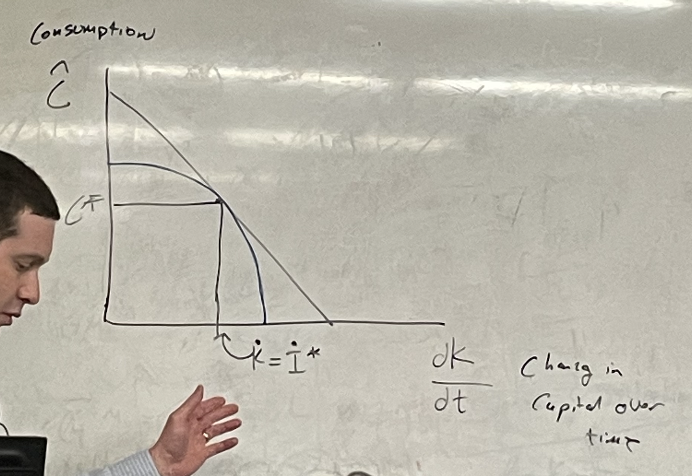
\includegraphics[width=14cm]{Screen Shot 2023-04-17 at 9.17.12 AM.png}
    \caption{Curved line is production possibilities frontier. }
\end{figure}

$C^*$ in Figure one is equivalent to thinking about the net national product. That is the consumption associated with non-declining wealth. \\

GDP is about flows and capital is about stocks. GDP has no thought about distribution because it is a single numbered metric. 


\section{The "real" issue with GDP}
There are arbitrary boundaries about what does and doesn't count as part of the economy. For example, while we don't measure drug sales and prostitution very well both, activities do technically count as GDP. Even though we aren't measuring these activities, that money eventually is laundered and hence added to production. \\

An area not included in GDP is household-related services. Cooking and cleaning don't count as a part of the GDP, but chopping wood or growing vegetables would be included in GDP. The things that don't count tend to be tasks that are historically associated with women. \\

There are also very strange boundaries around financial services. Innovation is also not well measured.  \\

Because GDP is the only single metric at the national scale, people use it as \textit{the metric} on national economic health. The Bureau of Economic Analysis repeatedly says you can't use GDP as a metric of wellbeing, but we should also hold them accountable to provide something better given that policy makers and citizens continue to think of GDP as a metric of national economic health. 

\section{Hartwick Rule}
Everyone working in the environment should understand the Hartwick Rule conceptually. Hartwick was a Canadian economist thinking about exhaustible resources in the 1970s and 80s. 

\begin{align}
    \max_{C, R} \int_0^\infty U(C) e^{-\delta t } dt
    s.t. \ \dot K = F(C, L, R) - C _ f(R,S)
\end{align}

where $C$ is consumption $R$ is resource extraction, $F(K,L,R)$ is the production function of the economy, $K$ is capital, $L$ is labor, and $f(R,S)$ is the cost of resource extraction and $S$ is the stock of resources. \\

We can now write a Hamiltonian with two state variables. 
\begin{align}
    H = U(C) - \lambda [F - C - f] - \mu R
\end{align}

FOCs (same basic Solow model):
\begin{align}
    \frac{\partial H}{\partial C}= U'(C) - \lambda =0 \label{solow}\\
    \implies 
    \frac{\partial H}{\partial R} = \lambda(F_R - f_R) - \mu = 0\\
    \implies \frac{\mu}{\lambda} = F_R - f_R \label{ratio}
\end{align}
\ref{solow} is the same result as the basic Solow model which says marginal utility equals the capital price of production of the resource. \\

Equation \ref{ratio}: The shadow price ratio is equal to the marginal value that the resource puts into production minus the rise in the cost of harvest/extraction of that resource. 

\begin{align}
    U(C) = U'(C) C \\
    \frac{H}{U'(C)} = C + \dot K - \frac{\mu}{\lambda} R \label{key_result}
\end{align}


$C + \dot K$ is net national product. $- \frac{\mu}{\lambda} R$ is the result of the Hartwick rule. This says that we must account for resource extraction. \\

\textbf{Hartwick Rule: }Resource rents need to be invested in some other form of production. If you sell capital goods, you can't count it as profit! \\

An example: Norway's sovereign wealth funds. \\

Another hot-take example: Yale taking the rents received from investments and oil then reinvesting it in scholarships for students (\textit{i.e.} Human Capital). \\

\section{Boundaries Issue of Capital}
What's in and what's out. \\


System of national accounts links 

\url{https://unstats.un.org/unsd/nationalaccount/snaupdate/wstt.asp}

\url{https://unstats.un.org/unsd/nationalaccount/towards2025.asp
}
 

National Strategy 

\url{https://www.whitehouse.gov/wp-content/uploads/2023/01/Natural-Capital-Accounting-Strategy-final.pdf
}
 

G7 Environment Ministerial

 \url{https://www.meti.go.jp/information/g7hirosima/energy/pdf/G7MinistersCommunique2023.pdf}

\url{https://www.meti.go.jp/information/g7hirosima/energy/pdf/Annex001.pdf}

\begin{figure}[htp]
    \centering
    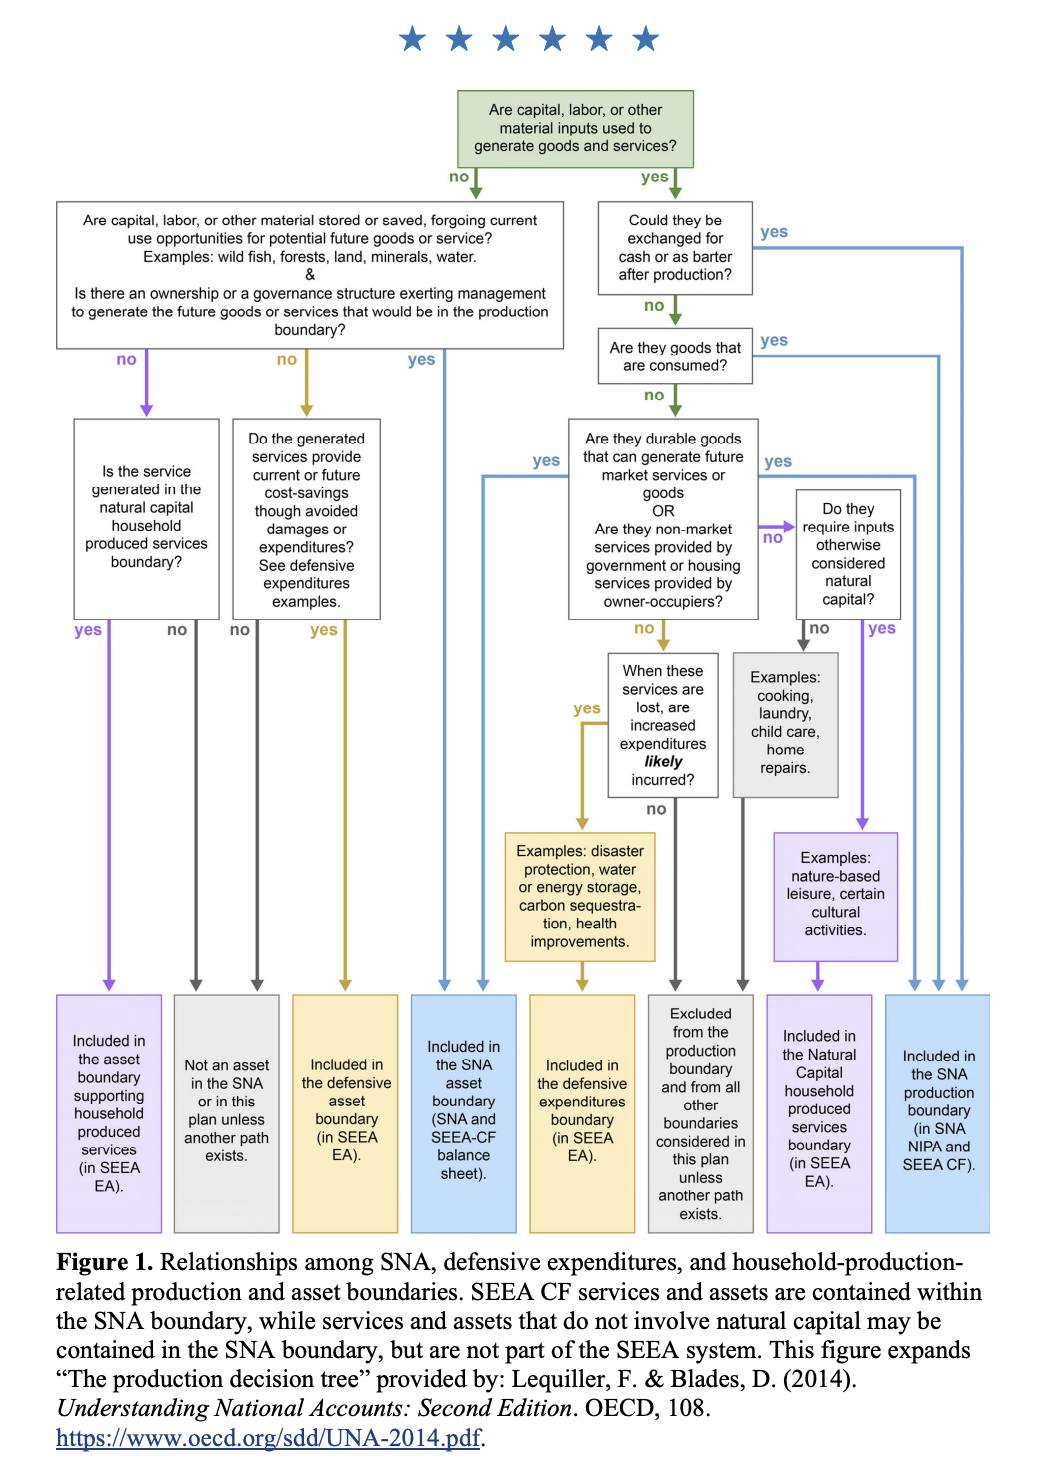
\includegraphics{Screen Shot 2023-04-17 at 10.15.08 AM.png}
    \caption{Caption}
    \label{fig:my_label}
\end{figure}

\end{document}